\begin{pastexam}[label={px:ust-106-ee-ds-10}]{臺聯大電機類 106 學年度 第十題}
（問答）

(10\%) Assume we have the following courses to take:

\begin{center}
\begin{tabular}{|l|l|l|l|}\hline
Course & Prerequisite & Course & Prerequisite\\\hline
CS150 & None & CS351 & CS151\\\hline
CS151 & CS150 & CS370 & CS151\\\hline
CS221 & CS151 & CS375 & CS151, CS222\\\hline
CS222 & CS221 & CS425 & CS325, CS222\\\hline
CS325 & CS221 & & \\\hline
\end{tabular}
\end{center}

Please draw a directed graph to show the relation between courses. A path from node $X$ to node $Y$ means
that you have to take course $X$ before course $Y$.
\end{pastexam}

\begin{pastsoln}
這是 AOV 網路（activity on vertex，資結書第~22.4~節）：每門課是一個頂點，「$X$ 是 $Y$ 的先修課」就
畫一條有向邊 $X \to Y$。 從表格逐列讀出邊：
\begin{center}
\begin{tabular}{ll}
\toprule
課程 & 指向它的邊 \\
\midrule
CS150 & 無（沒有先修） \\
CS151 & CS150 $\to$ CS151 \\
CS221 & CS151 $\to$ CS221 \\
CS222 & CS221 $\to$ CS222 \\
CS325 & CS221 $\to$ CS325 \\
CS351 & CS151 $\to$ CS351 \\
CS370 & CS151 $\to$ CS370 \\
CS375 & CS151 $\to$ CS375，CS222 $\to$ CS375 \\
CS425 & CS325 $\to$ CS425，CS222 $\to$ CS425 \\
\bottomrule
\end{tabular}
\end{center}
共 $9$ 個頂點、$10$ 條邊：

\begin{center}
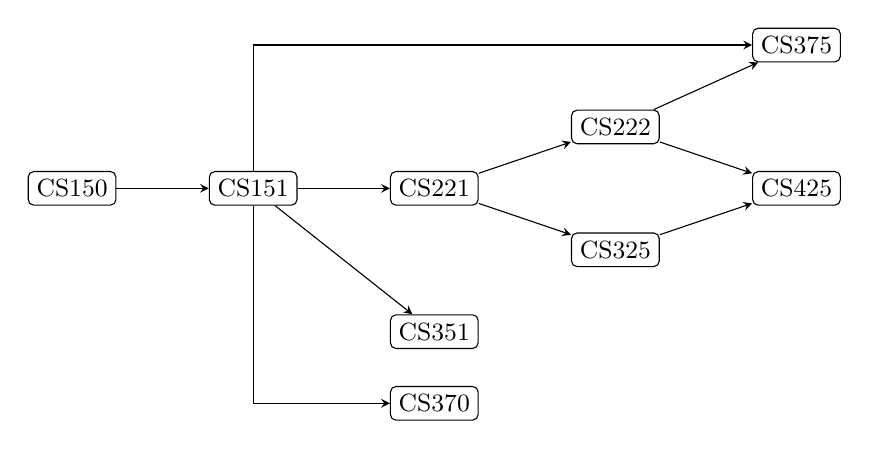
\begin{tikzpicture}[x=2.3cm,y=-1.3cm,>=stealth,
  every node/.style={draw,rounded corners=2pt,inner sep=3pt,font=\small}]
\node (a) at (0,1) {CS150};
\node (b) at (1,1) {CS151};
\node (c) at (2,1) {CS221};
\node (d) at (3,0.4) {CS222};
\node (e) at (3,1.6) {CS325};
\node (f) at (2,2.4) {CS351};
\node (g) at (2,3.1) {CS370};
\node (h) at (4,-0.4) {CS375};
\node (i) at (4,1) {CS425};
\draw[->] (a) -- (b);
\draw[->] (b) -- (c);
\draw[->] (c) -- (d);
\draw[->] (c) -- (e);
\draw[->] (b) -- (f);
\draw[->] (b) |- (g);
\draw[->] (b) |- (h);
\draw[->] (d) -- (h);
\draw[->] (d) -- (i);
\draw[->] (e) -- (i);
\end{tikzpicture}
\end{center}

\textbf{說明}。
\begin{itemize}
\item CS151 $\to$ CS375 這條邊，由 CS151 $\to$ CS221 $\to$ CS222 $\to$ CS375 已經推得出來（遞移），
但表格明白寫了 CS151 是 CS375 的先修，照表畫上去；省略它也不影響「哪些課要先修」。
\item 圖中沒有有向環（每條邊都從課號小的指向課號大的），所以一定排得出修課順序。 用 Kahn 演算法
（資結書第~22.1~節），每次取一門所有先修都修完的課，例如
CS150, CS151, CS221, CS222, CS325, CS351, CS370, CS375, CS425。
這只是其中一種拓樸順序，CS351、CS370 可以排在 CS151 之後的任何位置。
\end{itemize}
\end{pastsoln}
